\documentclass[main.tex,fontsize=8pt,paper=a4,paper=portrait,DIV=calc,]{scrartcl}
% Document
\usepackage[T1]{fontenc}
\usepackage[utf8]{inputenc}
\usepackage[dvipsnames]{xcolor}
\usepackage[nswissgerman,english]{babel} 
\usepackage{hyperref}
\renewcommand{\familydefault}{\sfdefault}

% Format
\usepackage[top=5mm,bottom=1mm,left=5mm,right=5mm]{geometry}
%\setlength{\headheight}{\baselineskip}
%\setlength{\headsep}{0mm}

%\usepackage{scrlayer-scrpage}
%\clearpairofpagestyles
%\chead{{\bfseries\TITLE, \AUTHOR, \pagename~\thepage}}

%\addtokomafont{pagehead}{\upshape}

\usepackage{multicol}
\setlength{\columnsep}{2mm}
\setlength{\columnseprule}{0.1pt}

% Math
\usepackage{amsmath}
\usepackage{amssymb}
\usepackage{amsfonts}

% Code
\usepackage{fancyvrb, etoolbox, listings, xcolor}
%\usemintedstyle{bw}

%\newminted[shell]{bash}{
%fontsize=\footnotesize,
%fontfamily=tt,
%breaklines=true,
%frame=single,
%framerule=0.1pt,
%framesep=2mm,
%tabsize=2
%}
%\newminted{css}{
%breaklines=true,
%tabsize=4,
%autogobble=true,
%escapeinside=||,
%stripall=true,
%stripnl=true,
%}

    \definecolor{lightgray}{rgb}{0.95, 0.95, 0.95}
    \definecolor{darkgray}{rgb}{0.4, 0.4, 0.4}
    \definecolor{purple}{rgb}{0.65, 0.12, 0.82}
    \definecolor{ocherCode}{rgb}{1, 0.5, 0} % #FF7F00 -> rgb(239, 169, 0)
    \definecolor{blueCode}{rgb}{0, 0, 0.93} % #0000EE -> rgb(0, 0, 238)
    \definecolor{greenCode}{rgb}{0, 0.6, 0} % #009900 -> rgb(0, 153, 0)
    \definecolor{teal}{rgb}{0.0, 0.5, 0.5}

\lstdefinestyle{code}{
    identifierstyle=\color{black},
    keywordstyle=\color{blue}\bfseries\small,
    ndkeywordstyle=\color{greenCode}\bfseries\small,
    stringstyle=\color{ocherCode}\ttfamily\small,
    commentstyle=\color{teal}\ttfamily\textit\small,
    basicstyle=\ttfamily\small,
    breakatwhitespace=false,         
    breaklines=true,                 
    captionpos=b,                    
    keepspaces=true,                 
    showspaces=false,                
    showstringspaces=false,
    showtabs=false,                  
    tabsize=2,
    belowskip=-5pt
}



% Images
\usepackage{graphicx}
\newcommand{\pic}{\includegraphics[scale=0.3]}
\graphicspath{{Screenshots/}{../Screenshots}}
\makeatletter
\def\pictext#1#2{%
    \@ifnextchar[{%
    \pictext@iiiii{#1}{#2}%
    }{%
      \pictext@iiiii{#1}{#2}[0.5,0.4,0.3]% Default is 5
    }%
}
\def\pictext@iiiii#1#2[#3,#4,#5]{\begin{minipage}{#3\textwidth}\includegraphics[scale=#4]{#1}\end{minipage}\begin{minipage}{#5\textwidth}#2\end{minipage}}
\def\minipg#1#2{%
    \@ifnextchar[{%
    \minipg@iiii{#1}{#2}%
    }{%
      \minipg@iiii{#1}{#2}[0.3,0.6]% Default is 5
    }%
}
\def\minipg@iiii#1#2[#3,#4]{\vspace{0.8mm}\begin{minipage}{#3\textwidth}#1\end{minipage}\begin{minipage}{#4\textwidth}#2\end{minipage}{\vspace{0.8mm}}}
\makeatother

%\newenvironment{minty}[2]% environment name
%{% begin code
%  \begin{minipage}{#1}
%  \begin{minted}{#2}
%}%
%{% end code
%  \end{minted}
%  \end{minipage}
%  \end{minty}\ignorespacesafterend
%} 

% Smaller Lists
\usepackage{enumitem}
\setlist[itemize,enumerate]{leftmargin=3mm, labelindent=0mm, labelwidth=1mm, labelsep=1mm, nosep}
\setlist[description]{leftmargin=0mm, nosep}
\setlength{\parindent}{0cm}

% Smaller Titles
\usepackage[explicit]{titlesec}

%% Color Boxes
\newcommand{\sectioncolor}[1]{\colorbox{black!60}{\parbox{0.989\linewidth}{\color{white}#1}}}
\newcommand{\subsectioncolor}[1]{\colorbox{black!50}{\parbox{0.989\linewidth}{\color{white}#1}}}
\newcommand{\subsubsectioncolor}[1]{\colorbox{black!40}{\parbox{0.989\linewidth}{\color{white}#1}}}
\newcommand{\paragraphcolor}[1]{\colorbox{black!30}{\parbox{0.989\linewidth}{\color{white}#1}}}
\newcommand{\subparagraphcolor}[1]{\colorbox{black!20}{\parbox{0.989\linewidth}{\color{white}#1}}}

%% Title Format
\titleformat{\section}{\vspace{0.5mm}\bfseries}{}{0mm}{\sectioncolor{\thesection~#1}}[{\vspace{0.5mm}}]
\titleformat{\subsection}{\vspace{0.5mm}\bfseries}{}{0mm}{\subsectioncolor{\thesubsection~#1}}[{\vspace{0.5mm}}]
\titleformat{\subsubsection}{\vspace{0.5mm}\bfseries}{}{0mm}{\subsubsectioncolor{\thesubsubsection~#1}}[{\vspace{0.5mm}}]
\titleformat{\paragraph}{\vspace{0.5mm}\bfseries}{}{0mm}{\paragraphcolor{\theparagraph~#1}}[{\vspace{0.5mm}}]
\titleformat{\subparagraph}{\vspace{0.5mm}\bfseries}{}{0mm}{\subparagraphcolor{\thesubparagraph~#1}}[{\vspace{0.5mm}}]

%% Title Spacing
\titlespacing{\section}{0mm}{0mm}{0mm}
\titlespacing{\subsection}{0mm}{0mm}{0mm}
\titlespacing{\subsubsection}{0mm}{0mm}{0mm}
\titlespacing{\paragraph}{0mm}{0mm}{0mm}
\titlespacing{\subparagraph}{0mm}{0mm}{0mm}

%% format cells
\usepackage[document]{ragged2e}
\usepackage{array, makecell}
\renewcommand{\arraystretch}{2}
\newcommand{\mc}{\makecell[{{m{1\linewidth}}}]}



\begin{document}
\tableofcontents

\newcommand{\TITLE}{Software Engineering Practises 2}
\newcommand{\AUTHOR}{Fabio Lenherr}
\setcounter{tocdepth}{1}

\section{Software Quality}
\subsection{Therac25 Rontgen overdosis (causes)}
\begin{itemize}
\item \textcolor{black}{unknown, single developer}
\item \textcolor{black}{reused parts by former employees without documentation}
\item \textcolor{black}{Bad UI -> misuse}
\item \textcolor{black}{bad documentation}
\item missing processes for identifying problems -> testing
\item missing processes for solving issues after accidents happen 
\item self written real-time OS instead of proven standard 
\item Software only tested with simulator, not with real hardware
\end{itemize} 

\subsection{Rules for Good Quality}
\begin{enumerate}
\item \textcolor{purple}{Conform to requirements}\newline
Write and test according to the customers needs, a smartphone app may crash, but a plane definitely not!
\item \textcolor{purple}{Use multiple layers of quality control}\newline
  Multiple layers of control will have a better chance of elmiminating the risk -> swiss cheese model
\end{enumerate} 

\subsection{Requirements}
\minipg{
\textcolor{purple}{Functional:}
\begin{itemize}
\item \textcolor{black}{acquired together with the customer}
\item \textcolor{black}{Userstories etc}
\item \textcolor{black}{easy to verify -> customer says yes}
\item WHAT does the system do?
\end{itemize} 
}{
\textcolor{purple}{Non-Functional:}
\begin{itemize}
\item \textcolor{black}{Defined by the customer AND the developer}
\item \textcolor{black}{Developer stories etc}
\item \textcolor{black}{Harder to verify}
\item \textcolor{black}{HOW does the system work? PSQL? GIN? BEVY?}
\end{itemize} 
}[0.25,0.25]

\subsubsection{Requirements Overview}
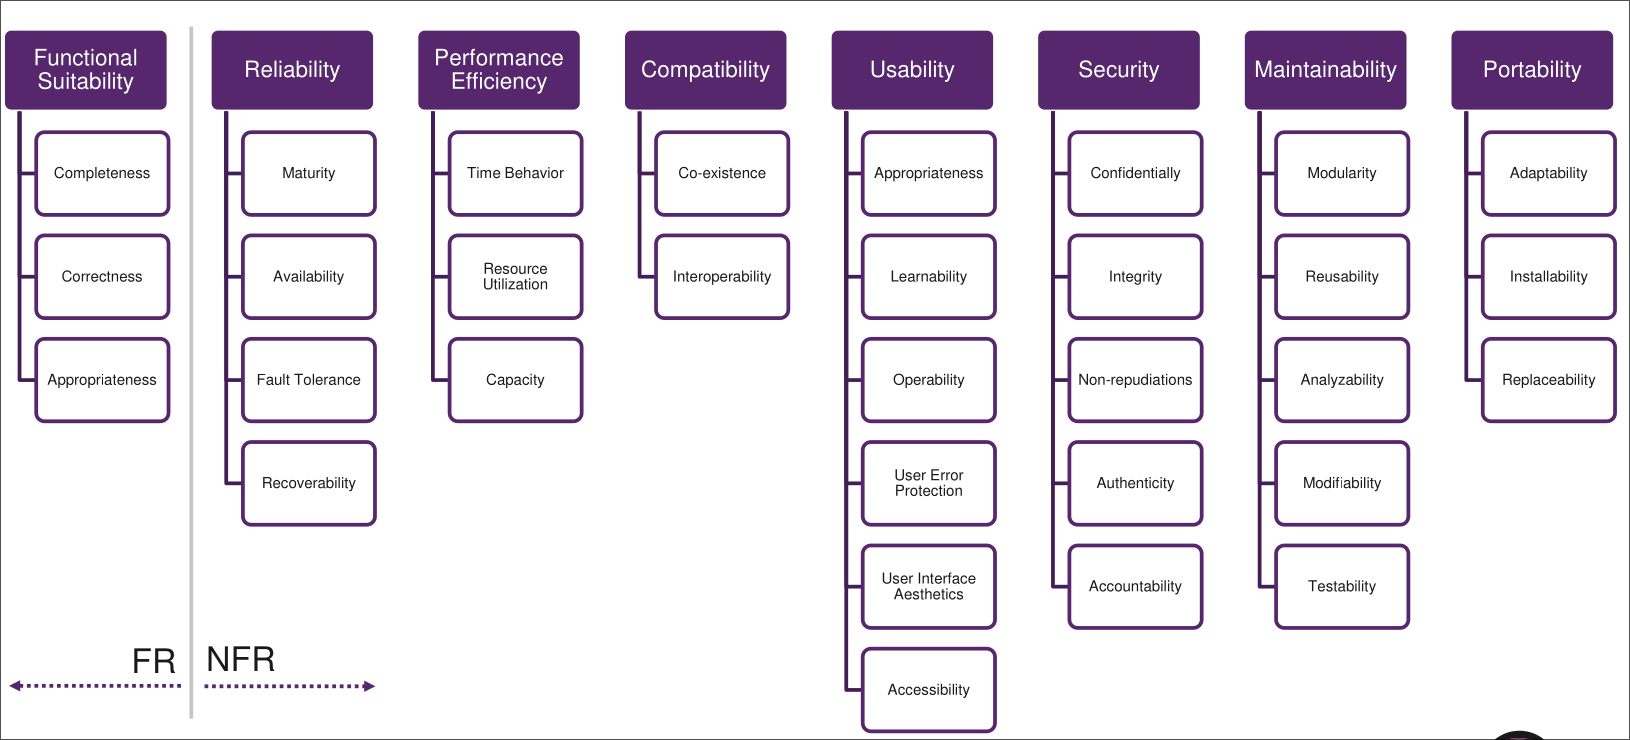
\includegraphics[scale=0.4]{2023_03_09_05_19_14.png}

\subsection{Overengineering and Underengineering}
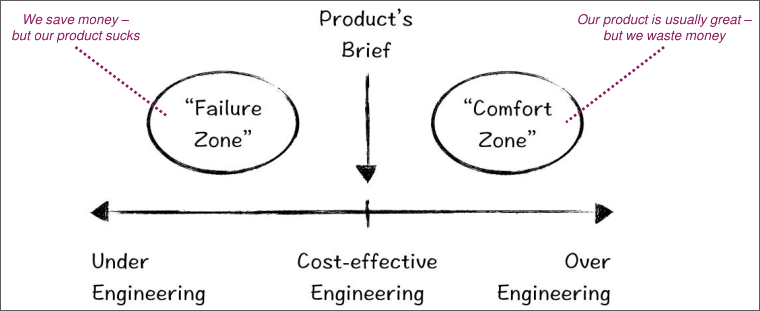
\includegraphics[scale=0.4]{2023_03_09_05_22_06.png}\newline
The right side wastes money, while the left side saves money at the cost of reputation.

\subsubsection{Technical Depth}
\textcolor{purple}{This is essentially just a backlog of things that you should still do. Ex. Tests, or better documentation, or a cleaner implementation.}\newline
Technical depth will often accumulate and you will end up at the left side, -> underengineering.\newline
It is important to keep track of this with developer stories and try to achieve \emph{more overengineering, rather than being complacent}.

\subsection{Software Aging}
\begin{itemize}
\item \textcolor{purple}{Causes}\newline
  \begin{itemize}
  \item \textcolor{black}{lack of change in technology}
  \item \textcolor{black}{update without thinking}
  \end{itemize} 
\item \textcolor{purple}{Costs}\newline
  \begin{itemize}
  \item \textcolor{black}{inability to keep up}
  \item \textcolor{black}{reduced performance}
  \item \textcolor{black}{decreasing reliability}
  \end{itemize} 
\item \textcolor{purple}{Remedy}\newline
  \begin{itemize}
  \item \textcolor{black}{stop the deterioration}
  \item \textcolor{black}{design for success}
  \item \textcolor{black}{plan ahead}
  \end{itemize} 
\end{itemize} 
\textcolor{red}{Important: Over time, the quality will pretty much always decline! -> wayland over Xorg!}

\subsubsection{Impact of complacency}
\textcolor{purple}{If you start to accept bugs, it will likely lead to more acceptence of more bugs. \newline
Eg. do not accept things such as not tested code, as it will likely reduce the quality of code in the long run!}

\subsubsection{Tools for Quality}
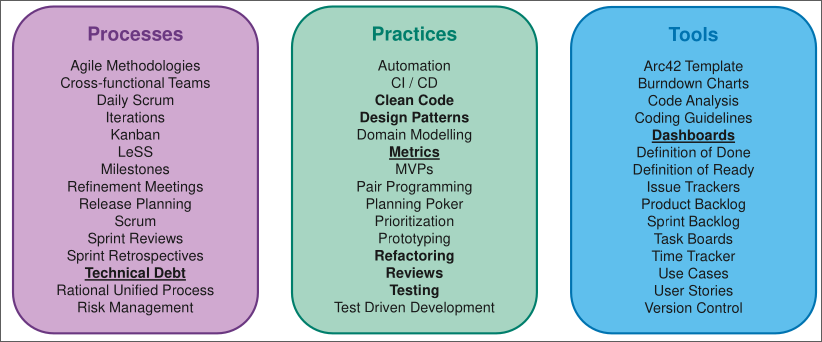
\includegraphics[scale=0.4]{2023_03_09_05_37_49.png}
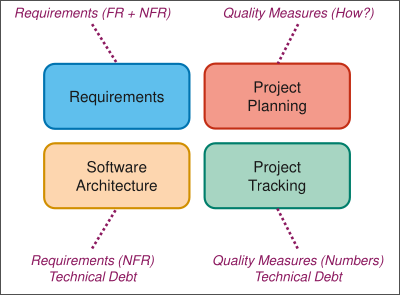
\includegraphics[scale=0.4]{2023_03_09_05_38_24.png}

\subsection{Maintainability of Code}
\begin{itemize}
\item \textcolor{purple}{POSIX function -> 1 functionality  per function}
\item \textcolor{purple}{Code Coverage}
\item \textcolor{purple}{Code Smells} LOC
\item \textcolor{purple}{Lines of code} CC
\item \textcolor{purple}{Cyclomatic Complexity} McCC
\end{itemize} 

\subsubsection{McCC}
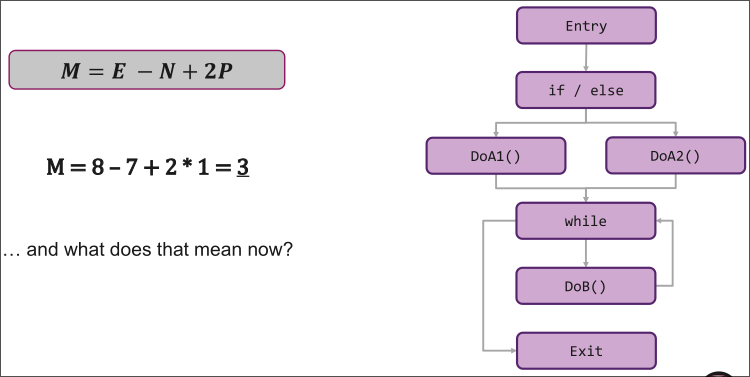
\includegraphics[scale=0.4]{2023_03_09_06_09_37.png}
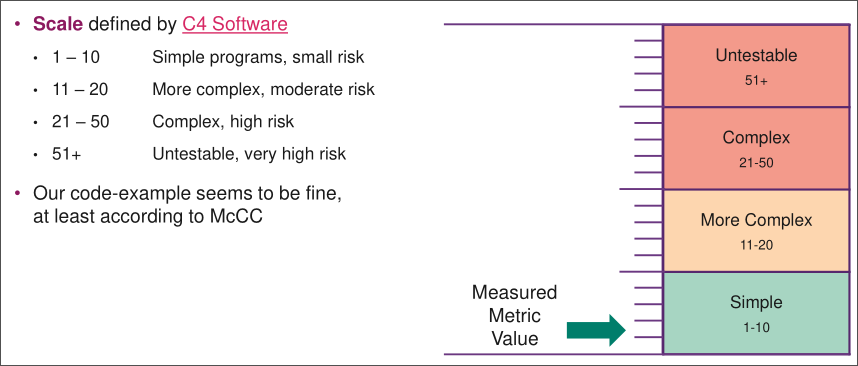
\includegraphics[scale=0.4]{2023_03_09_06_09_46.png}\newline
\textcolor{red}{Do NOT calculate this by hand, only let a tool do this task for you.}\newline
\textcolor{purple}{There are also a lot of tools that visualize the metric in order to stand out more to human eyes.}\newline
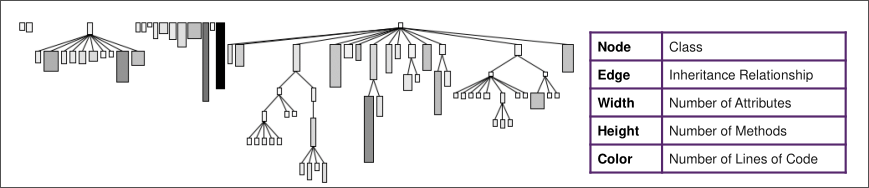
\includegraphics[scale=0.4]{2023_03_09_06_19_01.png}

\end{document}
